%%% CSE 4316 ADS - WORKED EXAMPLE (Mobile App + IoT). Follows ISO/IEC/IEEE 42010:2022 + IEEE 1016-2009.
\documentclass[11pt,letterpaper]{article}
\usepackage[margin=1.0in]{geometry}
\usepackage[T1]{fontenc}\usepackage[bitstream-charter]{mathdesign}\usepackage[latin1]{inputenc}
\usepackage{amsmath}\usepackage{xcolor}\usepackage{cite}\usepackage{hyphenat}
\usepackage{graphicx}\usepackage{float}\usepackage{subfigure}\usepackage{sectsty}
\usepackage[compact]{titlesec}\usepackage[tablegrid]{vhistory}\usepackage{pbox}\usepackage{longtable}
\usepackage{tikz}\usetikzlibrary{positioning,arrows.meta,fit,backgrounds}
\allsectionsfont{\color{accentcolor}\scshape\selectfont}
\definecolor{accentcolor}{rgb}{0.0,0.0,0.5}
\tikzset{
  mod/.style={draw, rounded corners, fill=white, minimum height=8mm, minimum width=27mm, font=\footnotesize, align=center, inner sep=2pt},
  ext/.style={draw, dashed, rounded corners, fill=black!4, minimum height=8mm, minimum width=24mm, font=\footnotesize\itshape, align=center, inner sep=2pt},
  band/.style={draw=accentcolor!45, rounded corners, inner sep=3.5mm},
  llbl/.style={font=\small\bfseries, text=accentcolor, align=left},
  flow/.style={-{Latex[length=2mm]}, thick, draw=accentcolor!80},
  fl/.style={font=\scriptsize, fill=white, inner sep=1pt},
}
\newcommand{\teamname}{Team Nimbus}
\newcommand{\productname}{AquaGuard Smart Water-Leak Monitor}
\newcommand{\coursename}{CSE 4316: Senior Design I}
\newcommand{\semester}{Fall 2026}
\newcommand{\docname}{Architectural Design Specification}
\newcommand{\department}{Department of Computer Science \& Engineering}
\newcommand{\university}{The University of Texas at Arlington}
\newcommand{\authors}{Alan Turing \\ Grace Hopper \\ John Von Neumann \\ Ada Lovelace \\ Charles Babbage}
\usepackage{fancyhdr}\pagestyle{fancy}\usepackage{lastpage}
\lhead{}\chead{}\rhead{}\lfoot{\footnotesize \teamname \ - \semester}\cfoot{}
\rfoot{\footnotesize page \thepage\ of \pageref{LastPage}}
\renewcommand{\headrulewidth}{0.0pt}\renewcommand{\footrulewidth}{0.4pt}
\usepackage[runin]{abstract}\abslabeldelim{\quad}\setlength{\abstitleskip}{-10pt}
\renewcommand{\abstractname}{}\renewcommand{\abstracttextfont}{\color{accentcolor} \small \slshape}

\begin{document}
{\centering \huge \color{accentcolor} \sc \textbf{\department \\ \university} \par}
\vspace{1 in}
{\centering \huge \color{accentcolor} \sc \textbf{\docname \\ \coursename \\ \semester} \par}
\vspace{0.5 in}
\begin{figure}[h!]\centering
\includegraphics[width=0.60\textwidth]{images/test_image}\end{figure}
\vspace{0.5 in}
{\centering \huge \color{accentcolor} \sc \textbf{\teamname \\ \productname} \par}
\vspace{0.5 in}{\centering \large \sc \textbf{\authors} \par}
\newpage
\begin{versionhistory}
  \vhEntry{0.1}{11.02.2026}{JVN}{document creation}
  \vhEntry{1.0}{11.18.2026}{AT|GH|CB}{official release}
\end{versionhistory}
\newpage\setcounter{tocdepth}{2}\tableofcontents\newpage

\section{Introduction}
Architecture of \productname\ as an ISO/IEC/IEEE 42010:2022 \cite{ISO42010}
description using IEEE 1016-2009 \cite{IEEE1016} viewpoints. Refines the SRS. Scope:
the sensor device, the mobile app, and the cloud backend.

\section{Stakeholders \& Architectural Concerns}
\begin{table}[H]\begin{center}\begin{tabular}{ | p{3.5cm} | p{9.5cm} |}\hline
\textbf{Stakeholder} & \textbf{Primary concerns} \\ \hline
Homeowner (user) & fast reliable alerts, easy setup, battery life \\ \hline
Advisor & product viability, cross-platform parity, cost \\ \hline
Development team & feasibility, BLE reliability, testability \\ \hline
Support/maintainers & diagnosability, OTA update path \\ \hline
\end{tabular}\end{center}\end{table}

\section{Architecture Viewpoints}
Context (Section 4), Composition/Data Flow (Section 5), Logical/Functional
(Sections 6--8), Deployment (Section 8). Style: an edge device (BLE peripheral) +
mobile central + cloud, with detection at the edge and alerting split between local
(BLE) and remote (push) paths. Interfaces \texttt{\#NN}; subsystems
\texttt{[Layer].[Name]}.

\section{System Overview \& Context View}
\begin{figure}[h!]\centering\resizebox{0.95\textwidth}{!}{%
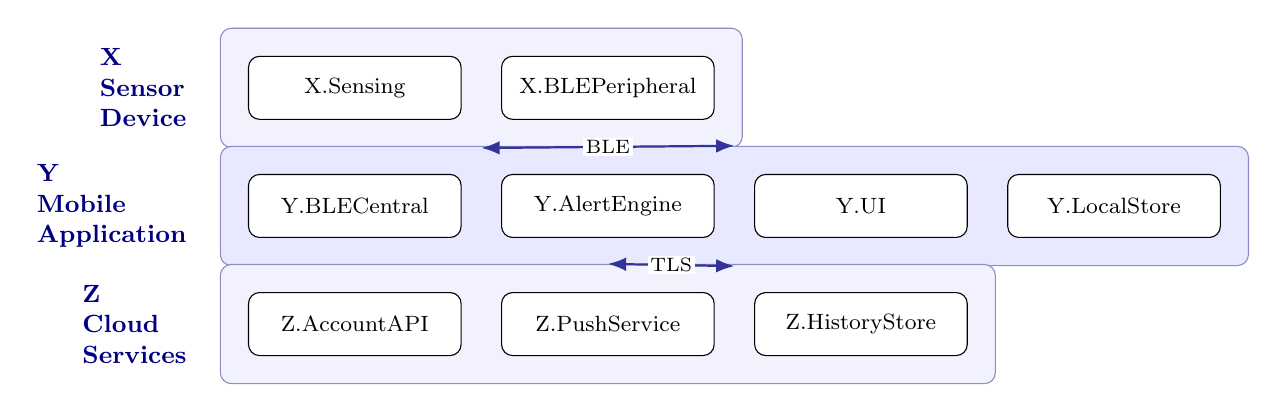
\begin{tikzpicture}[node distance=5mm]
\node[mod] (xsens) {X.Sensing};
\node[mod, right=of xsens] (xble) {X.BLEPeripheral};
\node[mod, below=15mm of xsens.west, anchor=west] (ybc) {Y.BLECentral};
\node[mod, right=of ybc] (yae) {Y.AlertEngine};
\node[mod, right=of yae] (yui) {Y.UI};
\node[mod, right=of yui] (yls) {Y.LocalStore};
\node[mod, below=15mm of ybc.west, anchor=west] (zapi) {Z.AccountAPI};
\node[mod, right=of zapi] (zpush) {Z.PushService};
\node[mod, right=of zpush] (zhist) {Z.HistoryStore};
\begin{scope}[on background layer]
\node[band, fill=blue!5, fit=(xsens)(xble)] (bx) {};
\node[band, fill=blue!9, fit=(ybc)(yls)] (by) {};
\node[band, fill=blue!5, fit=(zapi)(zhist)] (bz) {};
\end{scope}
\node[llbl, left=3mm of bx] {X\\Sensor\\Device};
\node[llbl, left=3mm of by] {Y\\Mobile\\Application};
\node[llbl, left=3mm of bz] {Z\\Cloud\\Services};
\draw[{Latex}-{Latex}, thick, draw=accentcolor!80] (bx.south) -- (by.north) node[fl,midway]{BLE};
\draw[{Latex}-{Latex}, thick, draw=accentcolor!80] (by.south) -- (bz.north) node[fl,midway]{TLS};
\end{tikzpicture}}
\caption{Three layers: sensor device, mobile app, cloud services}\end{figure}
External actors: the homeowner (phone UI) and the platform push services (APNs/FCM).
X senses and detects; Y connects, alerts locally, and relays; Z provides accounts,
history, and remote push.

\section{Subsystem Definitions \& Data Flow}
\begin{figure}[h!]\centering\resizebox{\textwidth}{!}{%
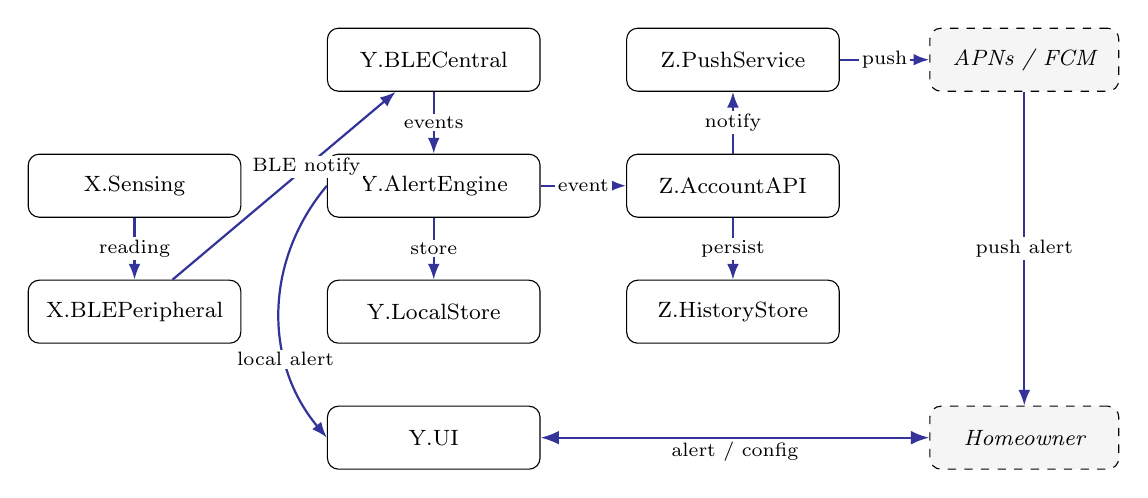
\begin{tikzpicture}
\node[mod] (xsens) at (2.6,0.8) {X.Sensing};
\node[mod] (xble)  at (2.6,-0.8){X.BLEPeripheral};
\node[mod] (ybc)  at (6.4,2.4) {Y.BLECentral};
\node[mod] (yae)  at (6.4,0.8) {Y.AlertEngine};
\node[mod] (yls)  at (6.4,-0.8){Y.LocalStore};
\node[mod] (yui)  at (6.4,-2.4){Y.UI};
\node[mod] (zpush) at (10.2,2.4){Z.PushService};
\node[mod] (zapi)  at (10.2,0.8){Z.AccountAPI};
\node[mod] (zhist) at (10.2,-0.8){Z.HistoryStore};
\node[ext] (apns) at (13.9,2.4){APNs / FCM};
\node[ext] (home) at (13.9,-2.4){Homeowner};
\draw[flow] (xsens) -- (xble) node[fl,pos=0.5]{reading};
\draw[flow] (xble) -- (ybc) node[fl,pos=0.6]{BLE notify};
\draw[flow] (ybc) -- (yae) node[fl,pos=0.5]{events};
\draw[flow] (yae) -- (yls) node[fl,pos=0.5]{store};
\draw[flow] (yae.west) to[bend right=40] node[fl,pos=0.68]{local alert} (yui.west);
\draw[flow] (yae) -- (zapi) node[fl,pos=0.5]{event};
\draw[flow] (zapi) -- (zpush) node[fl,pos=0.5]{notify};
\draw[flow] (zapi) -- (zhist) node[fl,pos=0.5]{persist};
\draw[flow] (zpush) -- (apns) node[fl,pos=0.5]{push};
\draw[flow] (apns) -- (home) node[fl,pos=0.5]{push alert};
\draw[{Latex}-{Latex}, thick, draw=accentcolor!80] (yui) -- (home) node[fl,pos=0.5,below]{alert / config};
\end{tikzpicture}}
\caption{Sensor $\rightarrow$ BLE $\rightarrow$ app $\rightarrow$ (local alert) / cloud $\rightarrow$ push}\end{figure}

\section{X Layer Subsystems --- Sensor Device}
\subsection{X.Sensing}
\textbf{Responsibilities:} sample moisture/flow and run on-device threshold detection
(FR-01) at low power (PE-01).
\begin{table}[H]\begin{center}\begin{tabular}{ | p{1cm} | p{6cm} | p{2.6cm} | p{2.6cm} |}\hline
ID & Description & Inputs & Outputs \\ \hline
\#01 & Sensor sampling & moisture/flow & reading, leak flag \\ \hline
\end{tabular}\end{center}\end{table}
\subsection{X.BLEPeripheral}
\textbf{Responsibilities:} expose the GATT profile (EI-01) --- live reading, leak
notify, threshold config, battery --- and manage bonded, encrypted links (SE-01).
\textbf{Rationale:} on-device detection keeps alerting working even if the phone is
briefly away and saves radio energy (AD-01).

\section{Y Layer Subsystems --- Mobile Application}
\subsection{Y.BLECentral}
\textbf{Responsibilities:} scan, pair/bond, subscribe to notifications, read/write
config (FR-02).
\begin{table}[H]\begin{center}\begin{tabular}{ | p{1cm} | p{6cm} | p{2.6cm} | p{2.6cm} |}\hline
ID & Description & Inputs & Outputs \\ \hline
\#02 & BLE central link & GATT notifications & events, config writes \\ \hline
\end{tabular}\end{center}\end{table}
\subsection{Y.AlertEngine}
\textbf{Responsibilities:} raise local visual/audible/haptic alerts (FR-03) and
forward events to the backend for remote push when disconnected (FR-04).
\subsection{Y.UI \& Y.LocalStore}
\textbf{Y.UI:} guided setup, live status, history (US-01, FR-05). \textbf{Y.LocalStore:}
on-device event/config cache; source for offline history.

\section{Z Layer Subsystems --- Cloud Services}
\subsection{Z.AccountAPI}
\textbf{Responsibilities:} device registration, user account, event ingestion over
TLS (SE-01). \textbf{Deployment:} small managed backend + database.
\subsection{Z.PushService}
\textbf{Responsibilities:} deliver alerts via APNs/FCM (EI-02, FR-04).
\subsection{Z.HistoryStore}
\textbf{Responsibilities:} durable event history (FR-05) synced with the app.

\section{Architecture Decisions \& Rationale}
\subsection{AD-01: Edge detection on the device}
\textbf{Context:} FR-01 latency + PE-01 battery + intermittent phone presence.
\textbf{Decision:} detect on the device, not in the app/cloud. \textbf{Alternatives:}
stream raw readings to the phone (higher radio energy, fails when away).
\textbf{Consequences:} firmware complexity up, energy/latency improved. \textbf{Affects:} FR-01, PE-01, FR-04.
\subsection{AD-02: Dual local/remote alert paths}
\textbf{Context:} FR-03 (nearby) and FR-04 (away). \textbf{Decision:} local BLE
alert plus cloud push fallback. \textbf{Alternatives:} push-only (slow when nearby),
BLE-only (no reach when away). \textbf{Consequences:} two paths to test. \textbf{Affects:} FR-03, FR-04.

\section{Requirements Traceability}
\begin{table}[H]\begin{center}\begin{tabular}{ | p{2cm} | p{5.5cm} | p{5cm} |}\hline
\textbf{Req ID} & \textbf{Requirement (abbrev.)} & \textbf{Realizing subsystem(s)} \\ \hline
FR-01 & Leak detection & X.Sensing \\ \hline
FR-02 & Pairing/config & Y.BLECentral, X.BLEPeripheral \\ \hline
FR-03 & Local alert & Y.AlertEngine \\ \hline
FR-04 & Remote alert & Y.AlertEngine, Z.PushService \\ \hline
FR-05 & History & Y.LocalStore, Z.HistoryStore \\ \hline
SE-01 & Secure pairing/TLS & X.BLEPeripheral, Z.AccountAPI \\ \hline
\end{tabular}\end{center}\end{table}

\bibliographystyle{reference/IEEEtran_custom}
\bibliography{reference/refs}{}
\end{document}
